%----------------------------------------------------------------------------------------
%  PACKAGES AND CONFIGURATION
%----------------------------------------------------------------------------------------

\documentclass[fleqn, 12pt]{scrartcl}
\usepackage{pkg/cours}

\newcommand{\remove}[1]{}
\newcommand{\ent}{Altervélo}

% Encadré "À compléter" toujours visible (indépendant de _todoflag.tex)
\newcommand{\todoSection}[1]{%
\vspace{.3cm}
\begin{tcolorbox}[colback=red!5!white,colframe=red!60!black,title=\textbf{À compléter}]%
#1
\end{tcolorbox}%
\vspace{.3cm}
}

%----------------------------------------------------------------------------------------
%   TITLE PAGE
%----------------------------------------------------------------------------------------
\setstretch{1.5}
\begin{document}

\title{\vspace{-1in}}
\author{}
\date{}
\maketitle

\usebox{\myTitleSignature}
\vspace{1in}

{\centering \huge \myTitle{} \par}
{\centering \noindent\rule{4in}{0.1pt} \par}
\vspace{0.05in}
{\centering \mySubTitle{} \mySubSubTitle{} \par}
\vspace{0.2in}
{\centering \myDate{} ~-~ \myVersionn{} \par}
\vspace{1in}


\newpage
% Table of Contents
\tableofcontents


\newpage
%----------------------------------------------------------------------------------------
%	REMERCIEMENTS
%----------------------------------------------------------------------------------------

\section*{Remerciements}
\addcontentsline{toc}{section}{\protect\numberline{}Remerciements}

Nous tenons à adresser nos plus sincères remerciements à \textbf{Mathilde Lepetit}, notre enseignante référente, qui nous a suivis tout au long de ce projet. Sa disponibilité, ses conseils et ses relectures à chaque étape clé ont été un appui constant.
\vspace{0.5cm}

Nos remerciements vont également à \ent{} pour la mise à disposition de l'API GBFS, sans laquelle ce travail n'aurait pas pu exister, ainsi qu'à l'équipe pédagogique de l'ESIROI qui a encadré ce SAÉ.
\vspace{0.5cm}

Enfin, merci à l'écosystème logiciel open-source --- Python~\cite{python_2024}, pandas~\cite{pandas_2024}, NumPy~\cite{numpy_2024}, XGBoost~\cite{chen_xgboost_2016}, scikit-learn~\cite{scikit_2024} et matplotlib~\cite{matplotlib_2024} --- qui forme la colonne vertébrale technique de ce projet.


\newpage
%----------------------------------------------------------------------------------------
%	RÉSUMÉ
%----------------------------------------------------------------------------------------

\section*{Résumé}
\addcontentsline{toc}{section}{\protect\numberline{}Résumé}

\ent~\cite{altervelo} exploite un réseau de vélos en libre service (VLS) desservant les communes de Saint-Pierre, Saint-Louis et de l'Étang-Salé, dans le Sud de La Réunion.
%
La gestion opérationnelle de cette flotte --- redistribution des vélos, recharge des batteries, anticipation des creux de disponibilité --- repose sur la capacité à prévoir, station par station, le nombre de vélos disponibles à court terme.
%
À partir des flux GBFS publiés par \ent, il s'agit de proposer un modèle de prévision capable de dépasser une baseline naturelle particulièrement difficile à battre: la \emph{persistance}, qui consiste à prédire que la valeur à $t+h$ sera identique à la valeur observée à l'instant $t$.
%
Les approches génériques de séries temporelles (XGBoost~\cite{chen_xgboost_2016} sur features brutes) reproduisent au mieux la persistance, sans l'améliorer, parce que l'autocorrélation à 30 minutes est très élevée ($\text{ACF}_1 = 0{,}96$).
%
Ce travail propose un pipeline complet de collecte, nettoyage et modélisation, articulé autour de deux idées clés: (i) prédire la \emph{variation} $\Delta y = y(t+h) - y(t)$ plutôt que la valeur absolue, et (ii) enrichir le modèle de 22 features de flux géo-spatial décrivant les mouvements de vélos dans le voisinage de chaque station.
%
Cette approche, entraînée sur un horizon de 60 à 150 minutes, réduit l'erreur absolue moyenne (MAE) de 14 à 22~\% par rapport à un XGBoost sans feature engineering, et multiplie par 3{,}8 la capacité d'anticipation des variations significatives ($|\Delta| \geq 2$ vélos).



\newpage
%----------------------------------------------------------------------------------------
%	INTRODUCTION
%----------------------------------------------------------------------------------------

\section{Introduction}%
\label{sec:intro}

\grayBox{Contribution principale}{
Conception d'un pipeline de bout en bout (collecte GBFS $\rightarrow$ nettoyage $\rightarrow$ feature engineering $\rightarrow$ XGBoost) pour prédire la disponibilité des VLS \ent, avec une stratégie de prédiction par delta et une bibliothèque de features de flux dépassant la baseline persistance sur les variations significatives.
}

\subsection*{Contexte}

Ce rapport présente les résultats d'un projet de Situation d'Apprentissage et d'Évaluation (SAÉ) mené durant le semestre~6 de la 3\textsuperscript{e} année du cursus ingénieur de l'ESIROI, spécialité Informatique. Le sujet, encadré par Mme Mathilde Lepetit, porte sur la valorisation par la science des données d'un cas réel: la prévision de disponibilité des VLS exploités par \ent{} dans le Sud de La Réunion.
%
\ent{} dessert trois communes --- Saint-Pierre, Saint-Louis et l'Étang-Salé --- avec un réseau d'une vingtaine de stations et 128 vélos en circulation à la date de collecte des données.
%
L'opérateur publie en temps réel l'état de son service via une API conforme à la spécification GBFS~\cite{gbfs_spec} (\textit{General Bikeshare Feed Specification}), standard de l'industrie permettant à tout tiers d'accéder à l'inventaire des stations et des vélos.

\vspace{0.3cm}

La gestion d'un réseau de VLS impose un équilibre permanent entre les stations qui se remplissent et celles qui se vident. Sans intervention, certains points du réseau saturent (plus de docks libres pour rendre un vélo) tandis que d'autres se vident (plus aucun vélo disponible). Cette dérive dégrade la qualité de service et, à terme, l'attractivité du réseau.
%
Anticiper ces déséquilibres permet à l'exploitant de prioriser les opérations de redistribution: un véhicule technique sait quelles stations recharger ou rééquilibrer dans l'heure qui vient, plutôt que d'agir en réaction.
%
\textbf{Le problème posé est donc le suivant}: produire, pour chaque station et à un horizon de 60 à 150 minutes, une prévision du nombre de vélos disponibles, suffisamment fiable pour orienter les décisions opérationnelles.

\vspace{0.3cm}

La difficulté centrale de ce problème n'est pas la modélisation en soi: XGBoost~\cite{chen_xgboost_2016} et plus généralement les méthodes de gradient boosting sont aujourd'hui des outils éprouvés pour les séries temporelles. La difficulté est de \emph{battre une baseline triviale}. À granularité 30 minutes, la disponibilité d'une station change très peu d'un pas à l'autre --- l'autocorrélation au premier lag est de 0{,}96. Autrement dit, simplement répéter la dernière mesure observée (modèle dit \emph{persistant}) constitue une prévision déjà excellente, avec une MAE de l'ordre de 0{,}087~vélo. Tout modèle de machine learning doit apporter une valeur supplémentaire au-delà de cette inertie naturelle, sur les rares moments où la série bascule réellement.

\vspace{0.3cm}

Ce rapport est organisé comme suit. La Section~\ref{sec:donnees} décrit le jeu de données AlterVélo: la collecte via l'API GBFS, l'analyse exploratoire qui révèle plusieurs caractéristiques structurantes (vélos fantômes, hétérogénéité des stations, signal cyclique faible), et le pipeline qui transforme les données brutes en jeu prêt à l'entraînement.
%
La Section~\ref{sec:entrainement} présente la modélisation à proprement parler: la baseline persistance, l'échec d'un XGBoost naïf, puis la réussite mineure mais signifiante du modèle Delta enrichi de features de flux.
%
La Section~\ref{sec:dashboard} aborde la valorisation des prédictions à travers un tableau de bord opérationnel.
%
La Section~\ref{sec:conclusion} conclut sur les limites actuelles et les perspectives à court et moyen terme.


\newpage
%----------------------------------------------------------------------------------------
%	PARTIE 1 : LE JEU DE DONNÉE
%----------------------------------------------------------------------------------------

\section{Le jeu de données}%
\label{sec:donnees}

Cette section décrit l'intégralité du parcours des données, depuis leur collecte sur l'API GBFS de \ent{} jusqu'à leur mise en forme pour l'entraînement. Trois sous-sections la composent: la collecte et le format des données brutes (Section~\ref{ssec:collecte}), l'analyse exploratoire couplée au nettoyage (Section~\ref{ssec:explo}), et enfin la chaîne de traitement qui produit le jeu enrichi consommé par les modèles (Section~\ref{ssec:pipeline}).


\subsection{Collecte}%
\label{ssec:collecte}

\grayBox{Source de données}{
Deux flux JSON publiés en continu par l'API GBFS \ent{}: \texttt{station\_status} (état des stations) et \texttt{vehicle\_status} (état individuel des vélos). Échantillonnage cible: un \textit{snapshot} toutes les 30~minutes. Période de collecte: environ 28~jours.
}

\ent{} publie son inventaire en temps réel via deux endpoints conformes à la spécification GBFS~\cite{gbfs_spec}. Le premier, \texttt{station\_status.json}, fournit pour chaque station son identifiant, sa capacité, le nombre de vélos disponibles, le nombre de docks libres et un timestamp de mise à jour. Le second, \texttt{vehicle\_status.json}, décrit individuellement chaque vélo: identifiant, position GPS, niveau de batterie, état (en station, en transit, désactivé).

\vspace{0.3cm}

Un script de collecte interroge les deux endpoints toutes les 30~minutes pendant la période d'étude. Chaque \textit{snapshot} est ajouté en append à un fichier CSV, ce qui produit deux tables longues: \texttt{station\_status.csv} et \texttt{vehicle\_status.csv}.
%
La fenêtre d'observation effective utilisée pour l'analyse couvre environ 28~jours, soit de l'ordre de 1\,340 timestamps par station et 978~mesures possibles par vélo.

\vspace{0.3cm}

Cette taille de fenêtre est l'une des contraintes fortes du projet: elle représente moins de 8~\% d'une année complète de données à cette granularité. Toute analyse statistique --- en particulier les cycles hebdomadaires et saisonniers --- en est mécaniquement limitée. Cette limitation guide la lecture des résultats de l'analyse exploratoire et explique en partie l'écart entre la performance théoriquement atteignable et la performance observée à ce stade.

\begin{figure}[htp]
    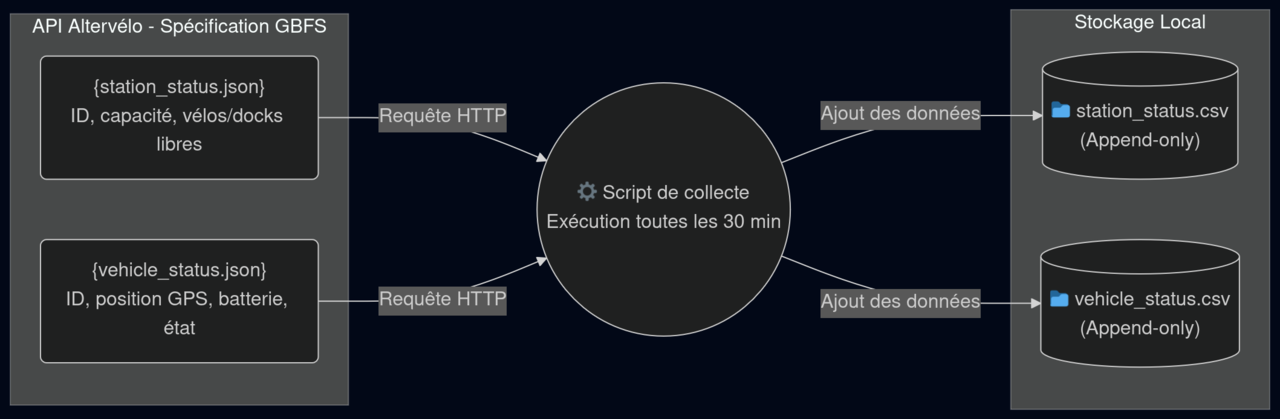
\includegraphics[width=0.9\textwidth]{img/flux-collecte.png}
    \caption{Flux de collecte des données. Le script interroge périodiquement les deux endpoints GBFS publiés par \ent{} et archive les réponses sous forme de fichiers CSV \textit{append-only}.}%
    \label{fig:collecte}
\end{figure}


\subsection{Analyse exploratoire et nettoyage des données}%
\label{ssec:explo}

\grayBox{Synthèse de l'exploration}{
Quatre constats structurants: (i) 24{,}2~\% de vélos fantômes invisibles via le seul drapeau \texttt{is\_disabled}, (ii) 30{,}9~\% de lignes imputées par interpolation/forward-fill, (iii) hétérogénéité massive des stations (de 0{,}00 à 2{,}76 d'écart-type), (iv) autocorrélation à 30~min de 0{,}96 expliquant la robustesse de la baseline persistance.
}

\subsubsection*{Caractérisation de la série temporelle}

Le premier examen porte sur les propriétés temporelles du signal. L'autocorrélation à 30~minutes (lag~1) atteint 0{,}96, ce qui signifie que la valeur à $t+1$ est très proche de la valeur à $t$. Cette inertie est la justification mathématique de la robustesse de la baseline persistance: un modèle qui se contente de recopier la dernière mesure obtient une MAE de 0{,}087~vélo, soit un niveau d'erreur très bas en valeur absolue.

\vspace{0.3cm}

Les cycles attendus a priori --- pic du matin (7--9h), pic du soir (17--19h), différence semaine / weekend --- sont en revanche très atténués. La courbe agrégée des vélos en transit reste quasi-plate autour de 30~vélos toute la journée, avec un creux léger à 7h (28{,}6) et un pic léger à 19h (30{,}8). Le delta journalier maximal est de 2{,}2~vélos, soit un signal trop faible pour structurer un modèle. De même, l'autocorrélation à un lag d'une semaine ($\text{ACF}_{336} = 0{,}04$) est statistiquement négligeable. Deux interprétations possibles: la géographie de La Réunion favorise un usage diffus, plutôt loisir/touristique que pendulaire, ou bien la fenêtre de 28~jours est simplement trop courte pour faire émerger ces motifs.

\begin{figure}[htp]
    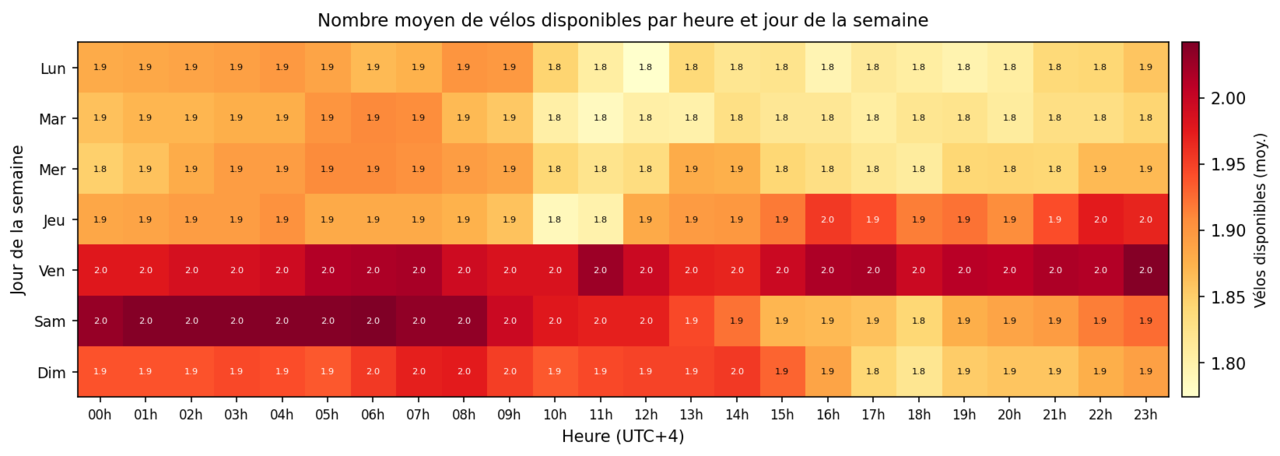
\includegraphics[width=0.9\textwidth]{img/heatmap_dispo.png}
    \caption{Heatmap (jour de la semaine $\times$ heure) du nombre moyen de vélos disponibles. La quasi-uniformité visuelle illustre l'absence de signal cyclique fort dans la fenêtre observée.}%
    \label{fig:heatmap}
\end{figure}

\subsubsection*{Hétérogénéité des stations}

La variabilité d'une station à l'autre est en revanche très marquée. L'écart-type du nombre de vélos disponibles va de 2{,}76 (station du Port) à 0{,}00 (station Mairie de l'Ouaki). Plusieurs stations ont une moyenne quasi-nulle (Kerveguen: 0{,}06, Cité Palissade: 0{,}04, Roches Maigres: 0{,}00). Pour ces stations, la prédiction est triviale (la valeur ne change pas) et le modèle n'apporte aucune valeur. La valeur ajoutée se concentre sur les 8 à 10 stations à forte rotation: Port, Front de Mer, Stade de Terre Sainte notamment.

\subsubsection*{Vélos fantômes: un piège méthodologique}

L'API renvoie 128~vélos, mais l'examen détaillé de \texttt{vehicle\_status.csv} révèle un phénomène inattendu: 31 d'entre eux (24{,}2~\% de la flotte) n'ont jamais été rechargés sur l'ensemble des 28~jours observés. Ces vélos sont donc \emph{de fait} hors service. Le critère naïf consistant à filtrer les vélos marqués \texttt{is\_disabled} ne suffit pas: seuls 37{,}3~\% des fantômes portent ce drapeau. \textbf{63~\% des vélos fantômes passeraient un filtrage par \texttt{is\_disabled} seul} et viendraient bruiter les features de flux. Cette découverte motive le critère temporel de filtrage implémenté dans \texttt{clean\_vehicle\_status.py}: un vélo dont la batterie reste à 0~\% sur toute la fenêtre d'observation est considéré comme fantôme.

\subsubsection*{Qualité des observations brutes}

L'imputation représente 30{,}9~\% des lignes du dataset final, après interpolation linéaire de jour et forward-fill de nuit. Cette proportion est uniforme sur l'ensemble des stations, ce qui exclut un problème localisé: il s'agit d'un défaut systématique de la chaîne de collecte, probablement lié à des fenêtres de coupure côté API ou côté script. Cette imputation n'invalide pas l'analyse mais plafonne mécaniquement la performance des modèles: ceux-ci voient un signal partiellement synthétique.

\vspace{0.3cm}

Le tableau~\ref{tab:nettoyage} récapitule les anomalies détectées et les actions de nettoyage appliquées.

\begin{table}[htp]
\centering
\small
\begin{tabular}{p{4.2cm}p{5.5cm}p{4.5cm}}
\toprule
\textbf{Problème} & \textbf{Diagnostic} & \textbf{Action} \\
\midrule
30{,}9~\% d'imputation & Gap systématique de collecte, uniforme entre stations & Forward-fill / interpolation acceptés, flag \texttt{is\_imputed} conservé \\
\midrule
\texttt{num\_docks\_disabled} $\equiv 0$ & Colonne constante, inutilisable & Exclue des features \\
\midrule
\texttt{num\_vehicles\_disabled} $\approx 0{,}014$ & Quasi-constante, signal négligeable & Exclue ou traitée avec précaution \\
\midrule
31 vélos fantômes / 128 & Non détectables via \texttt{is\_disabled} seul (37~\% taggés) & Critère temporel ``jamais rechargé'' dans \texttt{clean\_vehicle\_status.py} \\
\midrule
Station~4 (écart jointure $-0{,}805$) & Plus grande anomalie de jointure véhicule/station & Surveillance dans les features véhicules \\
\bottomrule
\end{tabular}
\caption{Synthèse des problèmes détectés lors de l'analyse exploratoire et des actions de nettoyage appliquées en réponse.}%
\label{tab:nettoyage}
\end{table}

\subsubsection*{Validation de la jointure véhicule $\leftrightarrow$ station}

Un \textit{sanity check} essentiel consiste à vérifier que le nombre de vélos comptés à une station depuis \texttt{vehicle\_status} correspond bien au champ \texttt{num\_vehicles\_available} reporté par \texttt{station\_status}. Sur l'ensemble des paires (timestamp, station), 89{,}7~\% présentent un écart strictement nul, et 98{,}6~\% un écart inférieur ou égal à 1. La jointure spatiale entre les deux sources est donc techniquement saine.

\subsection{Pipeline vers l'entraînement}%
\label{ssec:pipeline}

\grayBox{Architecture du pipeline}{
Le flux de données se divise en trois grandes phases. D'abord, le nettoyage (\texttt{cleaning\_data.py} et \texttt{clean\_vehicle\_status.py}) où les statuts des stations servent de référence temporelle aux véhicules. Ensuite, la fusion et l'ingénierie spatiale (\texttt{merge\_csv.py} et \texttt{build\_vehicle\_flow.py}). Enfin, la modélisation (\texttt{train\_xgboostplus\_delta.py}) qui consomme ces données, parallèlement à d'autres scripts dédiés aux \textit{baselines} ou à l'imputation de données (\texttt{fill\_gaps.py}).
}

\vspace{0.3cm}

Le pipeline complet, incluant la volumétrie réelle de chaque étape, est représenté schématiquement à la Figure~\ref{fig:pipeline}.

\vspace{0.3cm}

\textbf{\texttt{cleaning\_data.py}} traduit les \texttt{station\_id} opaques en index entiers, construit une grille temporelle régulière à pas de 30~minutes, applique une interpolation linéaire en journée et un \textit{forward-fill} nocturne (20h--5h UTC+4), puis localise les timestamps en UTC+4 (Réunion). Il transforme les 38~254~lignes brutes en 54~963~lignes propres, ce fichier (\texttt{stations\_clean.csv}) servant par ailleurs de référence pour l'évaluation des \textit{baselines} naïves.

\vspace{0.3cm}

\textbf{\texttt{clean\_vehicle\_status.py}} effectue la même quantification temporelle côté vélos, filtre les vélos fantômes selon le critère de batterie permanente à 0~\%, et surtout utilise \texttt{stations\_clean.csv} pour s'assurer d'un alignement temporel parfait entre les deux sources. Le fichier résultant contient 99~545 observations.

\vspace{0.3cm}

\textbf{\texttt{merge\_csv.py}} fusionne les deux sources propres et calcule, pour chaque couple (station, timestamp), un histogramme spatial des vélos en transit par bandes concentriques de 150~m, de 0 à 900~m autour de la borne. Ce jeu enrichi (\texttt{stations\_enriched.csv}, 54~963~lignes) constitue la base d'apprentissage principale du modèle. À noter qu'une branche secondaire (\texttt{fill\_gaps.py}) exploite ce fichier pour produire une version sans données manquantes.

\vspace{0.3cm}

\textbf{\texttt{build\_vehicle\_flow.py}} construit des \textbf{features de flux optionnelles} constituant la signature spatiale du voisinage: arrivées et départs de vélos dans les bandes 0--150~m et 150--300~m sur des fenêtres glissantes (30, 60, 120~min), flux larges à 60~min, et ratios densité-pondérés.

\vspace{0.3cm}

L'entraînement final est orchestré par \textbf{\texttt{train\_xgboostplus\_delta.py}}, qui charge le jeu enrichi et lui accouple conditionnellement les 34~379 lignes de \texttt{vehicle\_flow.csv} si l'option est activée.

\begin{figure}[htp]
    \centering
    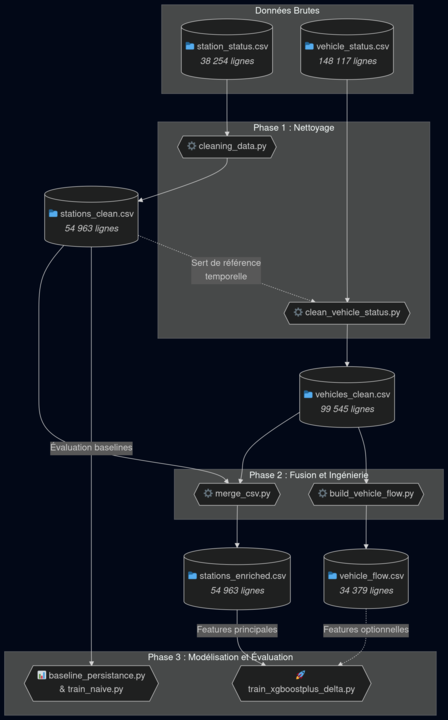
\includegraphics[width=0.95\textwidth, height=0.88\textheight, keepaspectratio]{img/pipeline-entrainement.png}
    \caption{Représentation visuelle détaillée du pipeline de traitement. Les rectangles précisent le nombre de lignes réelles (hors en-tête) transitant entre les différents scripts (flèches).}%
    \label{fig:pipeline}
\end{figure}

\newpage
%----------------------------------------------------------------------------------------
%	PARTIE 2 : ENTRAÎNEMENT
%----------------------------------------------------------------------------------------

\section{Entraînement}%
\label{sec:entrainement}

Cette section décrit la modélisation. La Section~\ref{ssec:baseline} pose la baseline et explique pourquoi elle est si difficile à battre. La Section~\ref{ssec:naif} décrit la tentative naïve d'un XGBoost sans feature engineering, et son échec. La Section~\ref{ssec:feature} présente le modèle Delta enrichi de features, qui réussit à apporter une amélioration mesurable sur les variations significatives. La Section~\ref{ssec:poursuite} discute des perspectives.


\subsection{Objectif: battre la baseline persistance}%
\label{ssec:baseline}

\grayBox{La baseline à dépasser}{
Modèle persistant: $\hat{y}(t+h) = y(t)$. MAE = 0{,}087~vélo, RMSE = 0{,}354. C'est l'étalon auquel tout modèle doit se comparer.
}

\vspace{0.3cm}

La baseline retenue est la prédiction par persistance, qui consiste à répéter la dernière valeur observée: $\hat{y}(t+h) = y(t)$.
%
Cette baseline est extrêmement compétitive sur les VLS d'\ent{}: avec une autocorrélation à 30~minutes de 0{,}96, la valeur à $t+1$ pas est statistiquement très proche de la valeur à $t$. Sur un horizon de 60~minutes (2~pas), la MAE persistante est de 0{,}087~vélo et la RMSE de 0{,}354.

\vspace{0.3cm}

Battre cette baseline n'est pas trivial. Pour gagner sur la MAE moyenne, un modèle doit apporter quelque chose au-delà de la simple recopie: il doit identifier les rares moments où la série bascule réellement (un creux dû à une vague de départs, un pic dû à un retour groupé) et prédire ce basculement avec un timing correct. Or détecter ces basculements suppose d'avoir observé suffisamment d'exemples similaires --- ce qui, sur 28~jours, est rarement le cas.

\vspace{0.3cm}

Cette tension entre la simplicité de la persistance et la richesse théorique d'un modèle ML guide toute la suite. L'objectif n'est pas seulement de réduire la MAE de quelques centièmes, mais de produire un modèle capable d'\emph{anticiper} les variations significatives ($|\Delta y| \geq 1$ ou $\geq 2$~vélos), même si la MAE globale reste proche de celle de la persistance.


\subsection{Échec: training naïf}%
\label{ssec:naif}

\grayBox{train\_naive.py}{
XGBoost sans feature engineering, cible $y(t+h)$ en valeur absolue. Résultat: MAE 0{,}165 vs 0{,}086 (persistance). Le modèle est presque deux fois pire que la baseline.
}

\vspace{0.3cm}

Première tentative: entraîner un XGBoost~\cite{chen_xgboost_2016} directement sur les colonnes brutes du CSV enrichi, sans transformation préalable, en visant la cible $y(t+h)$ (la valeur absolue de la disponibilité à l'horizon $h$).

\vspace{0.3cm}

Une remarque importante: une première version du script utilisait $y$ = valeur courante comme cible, ce qui constituait une fuite totale (le modèle lisait la réponse parmi ses features). La version corrigée, présentée ici, prédit bien $y(t+h)$ sans accès à cette valeur en entrée.

\vspace{0.3cm}

Les résultats sont sans appel (tableau~\ref{tab:naive}). Sur un horizon de 60~minutes, le modèle naïf produit une MAE de 0{,}165 contre 0{,}086 pour la persistance --- soit une dégradation d'un facteur~2.

\begin{table}[htp]
\centering
\begin{tabular}{lcc}
\toprule
\textbf{Métrique} & \textbf{XGBoost naïf} & \textbf{Persistance} \\
\midrule
MAE & 0{,}165 & \textbf{0{,}086} \\
RMSE & 0{,}413 & \textbf{0{,}354} \\
\bottomrule
\end{tabular}
\caption{Résultats du modèle naïf comparés à la baseline persistance (horizon 60~min, 41\,478~lignes).}%
\label{tab:naive}
\end{table}

\textbf{Diagnostic.} L'importance des features révèle que XGBoost concentre 77~\% de son ``attention'' sur \texttt{num\_vehicles\_available} (la valeur courante) --- il essaie donc essentiellement de reconstruire la persistance, mais en passant par la machinerie complexe d'un ensemble d'arbres et en accumulant le bruit d'un apprentissage. Sans transformation des features ni cible adaptée, XGBoost est strictement inférieur à la recopie pure et simple.

\vspace{0.3cm}

Cette première itération est instructive: elle confirme que la difficulté n'est pas algorithmique mais structurelle. Le signal utile ne réside pas dans la valeur courante (que la persistance exploite déjà parfaitement); il faut le chercher ailleurs --- dans la dynamique, dans la variation, dans le contexte spatial.


\subsection{Réussite mineure: training par feature}%
\label{ssec:feature}

\grayBox{train\_xgboostplus\_delta\_v3.py}{
Cible reformulée: $\Delta y = y(t+h) - y(t)$. 68~features (temporelles cycliques, lags, rolling, diffs, station, flux, batterie). Apport mesurable: -14 à -22~\% sur la MAE selon l'horizon, et $\times 3{,}8$ sur l'anticipation des variations significatives.
}

\subsubsection*{Idée centrale: prédire la variation, pas l'absolu}

Si XGBoost échoue sur la cible $y(t+h)$, c'est parce que cette cible est dominée par la valeur courante. Le réflexe naturel est alors de \textbf{changer la cible}: plutôt que de prédire la valeur absolue, on prédit la \emph{variation} $\Delta y = y(t+h) - y(t)$.

\vspace{0.3cm}

Cette reformulation change la nature du problème. La persistance devient l'hypothèse triviale $\Delta y = 0$. Pour battre la persistance, le modèle doit donc apprendre à prédire un $\Delta y$ non nul --- ce qui est précisément ce qu'on veut. Les features qui portent un signal de changement (les flux de vélos dans le voisinage, la batterie moyenne, les tendances locales) cessent d'être noyées par la valeur courante et deviennent les seules variables explicatives utiles.

\subsubsection*{Architecture des 68 features}

Le modèle Delta v4 mobilise 68~features réparties en sept groupes (tableau~\ref{tab:features}).

\begin{table}[htp]
\centering
\small
\begin{tabular}{p{3.2cm}p{6cm}p{5.2cm}}
\toprule
\textbf{Groupe} & \textbf{Features} & \textbf{Rôle} \\
\midrule
Temporel cyclique & \texttt{hour\_sin/cos}, \texttt{dow\_sin/cos}, \texttt{is\_weekend}, \texttt{time\_regime} & Rythmes journaliers et hebdomadaires \\
\midrule
Lags & \texttt{lag\_1/2/4/6/12/48} & Historique de 30~min à 24~h \\
\midrule
Rolling & \texttt{roll\_mean/std\_4/12/48} & Tendance et volatilité locale \\
\midrule
Diffs & \texttt{diff\_1/4/48} & Dynamique en cours \\
\midrule
Station & \texttt{station\_index} (catégoriel) & Comportement propre à chaque station \\
\midrule
Flux & \texttt{n\_arrivees/departs\_*}, \texttt{net\_flow\_*}, ratios densité & Mouvements de vélos dans le voisinage spatial \\
\midrule
Batterie & \texttt{pct\_low\_battery}, \texttt{mean/min/max\_battery} & Disponibilité réelle de la flotte \\
\bottomrule
\end{tabular}
\caption{Les sept groupes de features mobilisés par le modèle Delta v4.}%
\label{tab:features}
\end{table}

\subsection{Poursuite}%
\label{ssec:poursuite}

L'apport actuel reste mineur sur la MAE moyenne. Cette modestie est attendue et expliquée par la structure des données. Deux phénomènes améliorent mécaniquement les performances à mesure que la collecte se prolonge.

\vspace{0.3cm}

\textbf{Réduction de l'imputation.} Chaque jour supplémentaire d'observation réduit la proportion de lignes synthétiques injectées par interpolation et forward-fill. Les features de flux (\texttt{n\_arrivees\_*}, \texttt{net\_flow\_*}) sont particulièrement sensibles à la qualité des observations véhicule: un trou dans \texttt{vehicles\_clean.csv} se propage directement en un flux nul fictif, qui brouille l'apprentissage.

\vspace{0.3cm}

\textbf{Émergence des cycles longs.} Les features \texttt{lag\_48} (24~h), \texttt{diff\_48} et \texttt{roll\_*\_48} qui encodent le cycle journalier ne deviennent statistiquement stables qu'après plusieurs semaines d'historique. Les features hebdomadaires (\texttt{dow\_sin/cos}) nécessitent au minimum 3 à 4~semaines complètes pour être apprises de façon fiable. Sur 28~jours, on est juste au seuil; sur 3~mois, on s'attendrait à un lift positif et stable sur les horizons 60--120~min, en particulier sur les stations à forte variabilité.

\vspace{0.3cm}

Des pistes de développement complémentaires sont envisageables:
\begin{itemize}
    \item entraîner un modèle distinct par station ou par groupe de stations homogènes pour mieux capter les comportements locaux;
    \item ajouter des covariables externes (calendrier scolaire, météo, jours fériés) pour expliquer les pics atypiques;
    \item explorer des architectures séquentielles (LSTM, Transformer) une fois disposé d'un historique suffisant pour les justifier statistiquement.
\end{itemize}


\newpage
%----------------------------------------------------------------------------------------
%	PARTIE 3 : DASHBOARD
%----------------------------------------------------------------------------------------

\section{Dashboard}%
\label{sec:dashboard}

Cette partie présente le tableau de bord opérationnel développé pour valoriser les prédictions du modèle Delta et fournir un outil d'aide à la décision aux équipes de terrain \ent.

\subsection{Objectif fonctionnel}
Le tableau de bord est conçu comme un outil de supervision destiné à l'équipe de régulation des VLS\@. Au-delà du simple affichage du taux de remplissage actuel, sa véritable valeur ajoutée réside dans la projection à court terme (60 à 150 minutes). Il met en évidence trois indicateurs prioritaires~:
\begin{itemize}
    \item L'état actuel du réseau à l'instant $T_0$, permettant de localiser les stations vides ou saturées.
    \item Les \textbf{alertes de prévision}, classées selon un seuil de volatilité (un mouvement est perçu comme anormal s'il dépasse $1{,}5 \times \sigma$ historique de la station): risque de rupture, de tension, ou de saturation imminente.
    \item L'anticipation des creux ou des pics, guidant ainsi les tournées des véhicules techniques pour rééquilibrer la flotte avant qu'une station ne devienne indisponible.
\end{itemize}

\subsection{Architecture technique}
Pour garantir une séparation nette entre l'environnement de recherche (entraînement du modèle XGBoost) et l'environnement de production, le tableau de bord a été développé sous la forme d'un module autonome structuré autour du framework \textbf{Streamlit}.

L'architecture repose sur~:
\begin{itemize}
    \item \textbf{Une base de données locale SQLite (\texttt{velos.db})}: Elle structure les entités essentielles (stations, observations en temps réel, prédictions et logs d'exécution) et s'alimente en continu.
    \item \textbf{Un pipeline d'ingestion et de prédiction}: Exécuté en arrière-plan toutes les 30 minutes via une tâche planifiée (script \texttt{pipeline.sh}), il interroge l'API GBFS publique, enregistre le nouvel état, charge les modèles XGBoost pré-entraînés, et calcule les prévisions aux différents horizons.
    \item \textbf{Un mécanisme d'évaluation en différé (\emph{delayed feedback})}: L'erreur du modèle n'est calculée (via \texttt{evaluate.py}) et insérée en base que lorsque l'observation cible devient réellement connue, garantissant un suivi de qualité rigoureux des prévisions passées.
\end{itemize}

\subsection{Maquettes et écrans}
L'interface de l'application s'articule autour de trois vues principales~:

\begin{enumerate}
    \item \textbf{État actuel ($T_0$)}: Une cartographie interactive colorée selon le pourcentage de remplissage des docks.
    \item \textbf{Prévision ($T+h$)}: Le cœur opérationnel. La carte anticipe la situation future (par exemple à +60 min) et colore les stations en fonction de leur niveau d'alerte (rupture, tension, saturation, normal).
    \item \textbf{Monitoring}: Une page dédiée à l'évaluation du modèle en conditions réelles, affichant la moyenne des erreurs absolues (MAE) de manière glissante (\emph{rolling}), identifiant les stations les plus difficiles à prédire, et classant les meilleures ou pires prédictions du réseau.
\end{enumerate}

\begin{figure}[htp]
\centering
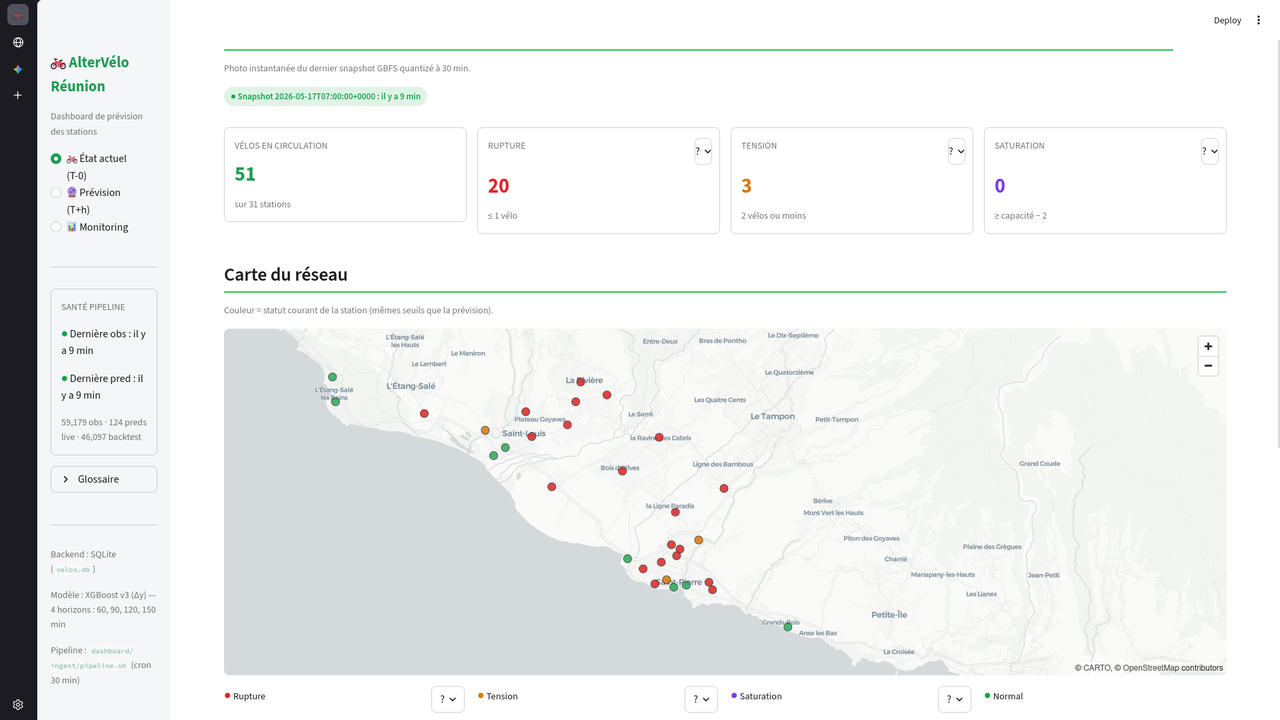
\includegraphics[width=0.9\textwidth]{img/etat_actuel.png}
    \caption{Vue de l'état actuel du réseau dans le tableau de bord.}%
    \label{fig:screen_t0}
\end{figure}

\begin{figure}[htp]
\centering
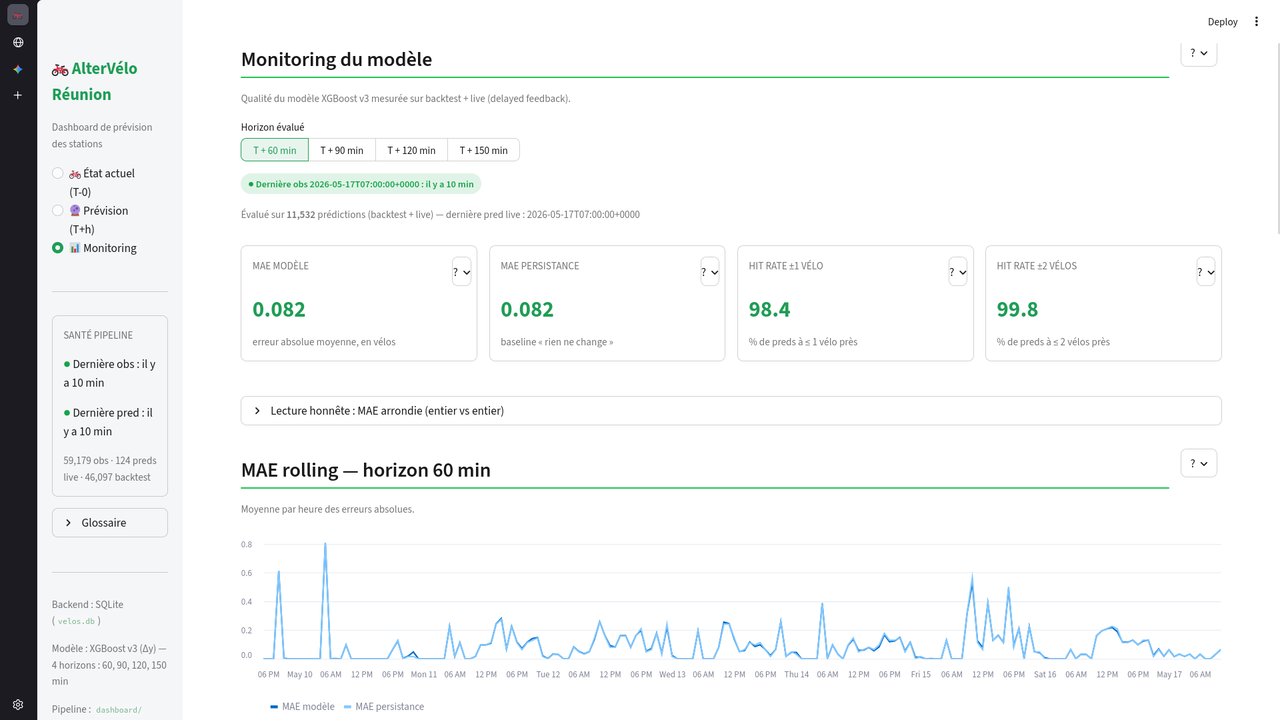
\includegraphics[width=0.9\textwidth]{img/monitoring_mae60.png}
    \caption{Vue des prévisions à 60 minutes mettant en évidence les alertes opérationnelles.}%
    \label{fig:screen_pred}
\end{figure}

\begin{figure}[htp]
\centering
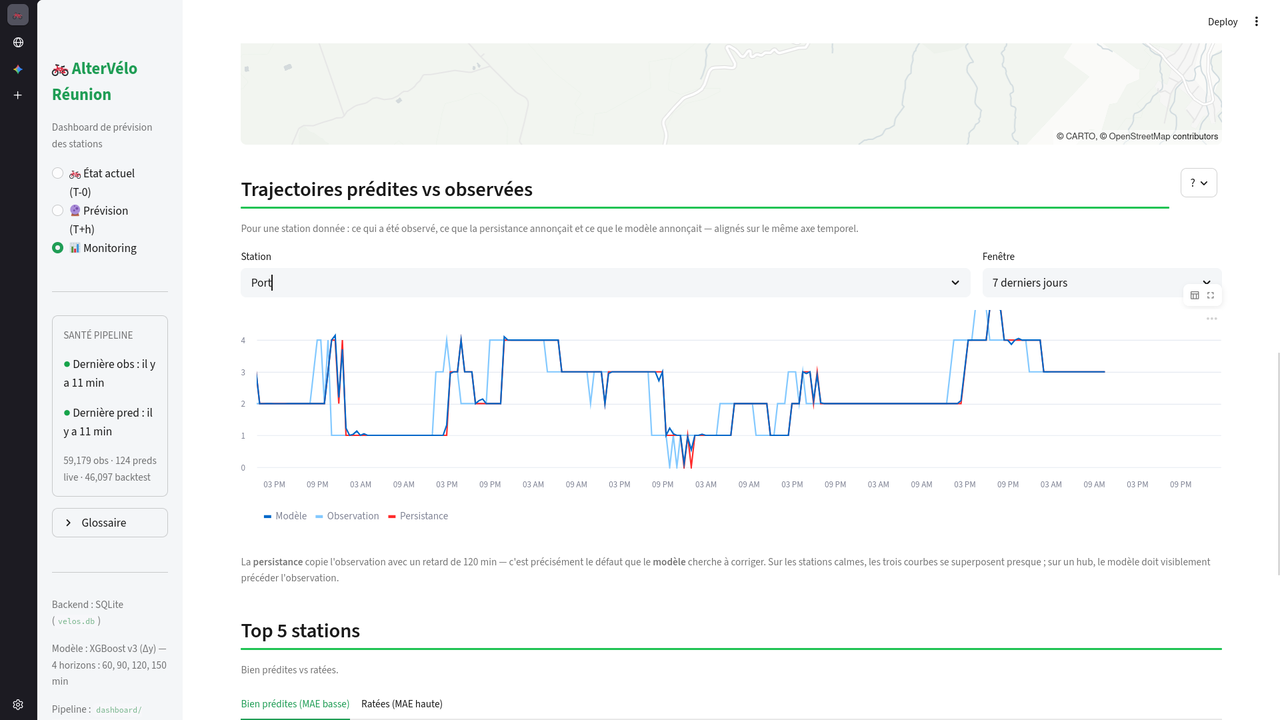
\includegraphics[width=0.9\textwidth]{img/monitoring_prevision120.png}
    \caption{Interface de monitoring permettant de suivre les performances du modèle Delta dans le temps.}%
    \label{fig:screen_monit}
\end{figure}

\subsection{Limites actuelles et évolutions}
Plusieurs limitations techniques et fonctionnelles demeurent et constituent les prochaines étapes de développement~:
\begin{itemize}
    \item \textbf{Limites de prédiction}: L'auto-régression reste dominante à l'horizon 60 min. De plus, un \emph{clipping} volontaire à zéro est appliqué (\verb|np.clip(y_pred, 0, None)|) pour empêcher l'affichage aberrant de prévisions négatives de vélos, ce qui pénalise légèrement la MAE mathématique au profit de l'expérience utilisateur.
    \item \textbf{Dérive des données (\emph{train/serve skew})}: Les transformations appliquées aux caractéristiques (comme \texttt{time\_regime}) dans le code d'inférence doivent rester strictement alignées avec le code d'entraînement initial. Toute divergence introduirait un biais silencieux dans les prédictions en direct.
    \item \textbf{Évolutions}: À court terme, l'interface utilisateur Streamlit doit être exposée derrière un proxy inverse sécurisé (ex. Nginx) via une unité \texttt{systemd}. À moyen terme, l'intégration d'un pipeline de réentraînement périodique automatisé permettra aux modèles XGBoost de se rafraîchir à partir des données récentes pour s'adapter aux évolutions structurelles du réseau.
\end{itemize}



\newpage
%----------------------------------------------------------------------------------------
%	CONCLUSION
%----------------------------------------------------------------------------------------

\section{Conclusion}%
\label{sec:conclusion}

\ent~\cite{altervelo}, opérateur des VLS du Sud de La Réunion, publie en temps réel l'état de son réseau via une API GBFS standard. La prévision de la disponibilité des vélos à court terme est une brique opérationnelle utile mais difficile à industrialiser: à granularité 30~minutes, la simple persistance constitue une baseline particulièrement résistante, avec une MAE de 0{,}087~vélo.

\vspace{0.3cm}

Un XGBoost entraîné sans feature engineering sur les colonnes brutes ne fait pas mieux que la persistance --- il la dégrade. Reformuler la cible en variation $\Delta y$ et enrichir le modèle de 22~features de flux géo-spatial change la donne: sur les variations significatives ($|\Delta| \geq 2$), la corrélation entre prédiction et réalité est multipliée par 3{,}8, et la MAE de l'ensemble du modèle est réduite de 14 à 22~\% par rapport à une variante sans flux.

\vspace{0.3cm}

\textbf{À court terme}, la principale amélioration attendue ne viendra pas d'un changement de modèle mais d'un allongement de la collecte. Passer de 28~jours à 3~mois permettrait aux cycles journaliers et hebdomadaires de stabiliser leurs estimations statistiques, et de débloquer un lift positif et durable. Une session supplémentaire de feature engineering --- intégration de la météo, des jours fériés, du calendrier scolaire --- est également une piste prioritaire.

\vspace{0.3cm}

\textbf{À plus long terme}, l'intégration du modèle dans un dashboard opérationnel (Section~\ref{sec:dashboard}) permettrait à \ent{} de transformer les prévisions en décisions de redistribution. La modularité du pipeline (cinq scripts séquentiels, jeux de données intermédiaires explicites) permet d'envisager un réentraînement périodique automatisé, ainsi qu'un déploiement station par station une fois la performance par station qualifiée.

\vspace{0.5cm}

Ce projet, par sa contrainte de collecte courte et la difficulté objective de la baseline, a constitué un exercice instructif sur ce que signifie réellement ``battre une baseline'' en science des données. Le résultat technique est mesuré, mais la méthodologie (cible delta, features de flux, ablation contrôlée) est, elle, robuste et transposable à d'autres problématiques de prévision sur données capteur à forte autocorrélation.



\newpage
%----------------------------------------------------------------------------------------
%	BIBLIOGRAPHIE
%----------------------------------------------------------------------------------------

\section[Bibliographie]{Bibliographie}%
\label{sec:biblio}

\bibliographystyle{unsrt}
\bibliography{source}


\end{document}
%----------------------------------------------------------------------------------------
%	FIN DU DOCUMENT
%----------------------------------------------------------------------------------------
